\section{Wirtualizacja i orkiestracja}

\subsection{Wirtualizacja - początki}
Opisując automatyzację procesów w przemyśle IT konieczne jest opisać wirtualizację czyli kolejny kamień milowy w budowie infrastruktury oraz współczesny sposób wytwarzania i dostarczania oprogramowania. Czym tak właściwie jest wirtualizacja? 
Żeby dobrze zrozumieć jak istotną rolę odgrywa wirtualizacja w automatyzacji warto spojrzeć wstecz i przyjrzeć się historii serwerów i komputerów w ogóle.   Jak podaje Paul E. Ceruzzi czyli autor książki "A History of Modern Computing"\cite{Computing}, w przeszłości jeśli była potrzeba uruchomienia serwera, były zasadniczo dwie opcje: 
\begin{itemize}
    \item zbudować swój własny fizyczny serwer,
    \item wynająć/kupić sprzęt komputerowy od firmy, która takie usługi prowadzi.
\end{itemize}
W pierwszym przypadku budowanie własnego serwera wymaga dużej liczby inżynierów z odpowiednią wiedzą i doświadczeniem, narzędzi oraz materiałów do budowy. Nie każda firma będzie więc spełnić te wszystkie wymagania, dlatego druga opcja stała się więc zdecydowanie bardziej popularna. Pierwszą firmą która skorzystała na trudzie wykonania własnego serwera była firma IBM i tak w 1960 powstał IBM Mainframe, czyli sprzęt najwyższej klasy jak na  ówczesne możliwości.

\begin{figure}[htbp]
    \centering
    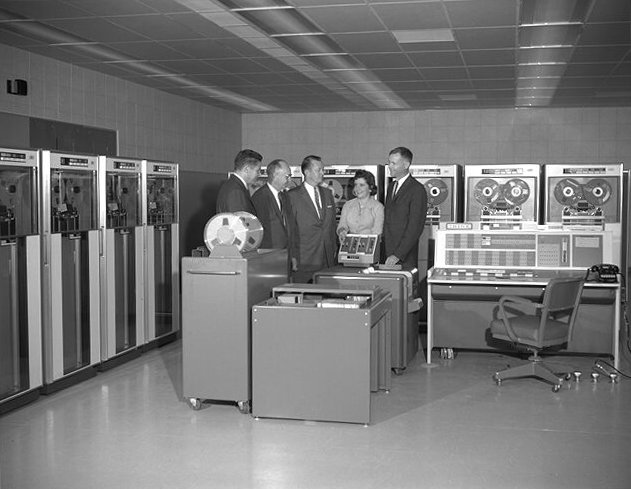
\includegraphics[width=10cm]{IBM-computer.jpg}
    \caption{IBM Mainframe}
    \label{fig:ibm-mainframe}
\end{figure}

Przez kolejne 20 lat sprzęty komputerowe firmy IBM dominowały rynek. Początkowo na Mainframie można było uruchomić tylko jedną aplikację, co powodowało duże marnowanie zasobów i czasu. Później została dodana wielozadaniowość co znacznie usprawniło działanie sprzętu. W 1980 roku był wielki "boom" technologiczny, który testował możliwości serwera. Szybko się okazało, że utrzymanie serwerów jest kosztowne. Konserwacja sprzętu, miejsce w którym serwery są przechowywane oraz koszty związane z administrowaniem sprawiły, że na rynku pojawiła się potrzeba na technologie wirtualizacyjne i tak w latach 90 XX wieku w wyniku połączenia wydajnych procesów oraz znawców z dziedziny sprzętu komputerowego powstały wirtualne maszyny i wirtualizacja w ogóle. 

\subsection{Czym są wirtualne maszyny?}
Wirtualne maszyny są kolejną warstwą abstrakcji między użytkownikiem a "metalem", czyli fizycznym sprzętem. Dzięki wykorzystaniu tego mechanizmu, zamiast jednego systemu operacyjnego uruchomionego na komputerze, możliwe jest uruchomienie wielu "gości" systemu operacyjnego na bazowym systemie operacyjnym. Dlaczego to jest takie przydatne? Teraz posiadając jedną mocną maszynę możemy dowolnie dodawać i usuwać serwery. Tak wiec jeśli  teraz dodamy dodatkową funkcjonalność do naszego programu, jedyne co należy zrobić żeby go wdrożyć jest dodanie dodatkowej wirtualnej maszyny na jednym z serwerów, który ma wystarczająco dużo miejsca, żeby to zrobić. To rozwiązanie daje bardzo dużo elastyczności. 
Jak dokładnie działa zarządzanie zasobami na wirtualnej maszynie?
Mechanizm dzięki któremu jest możliwa wirtualizacja nazywa się hypervisor. Hypervisor zarządza całym cyklem życia oraz funkcjonalnością wirtualnej maszyny. 
Do jego głównych zadań należą:
\begin{itemize}
    \item alokacja odpowiedniej ilości RAM'u, mocy obliczeniowej, pamięci dyskowej oraz zarządzanie połączeniem z siecią,
    \item startowanie wirtualnej maszyny,
    \item czyszczenie zasobów po zatrzymaniu wirtualnej maszyny,
    \item zapewnianie izolacji dla działających wirtualnych maszyn,
    \item zarządzanie wirtualnymi maszynami.
\end{itemize}
oraz wiele innych. 
Tak wiec podsumowując, jest jeden bazowy system operacyjny uruchomiony na komputerze, który udostępnia zasoby serwera wirtualnym maszynom i jeśli zasoby na tej wirtualnej maszynie się wyczerpią to nie ma to żadnego wpływu na inne wirtualne maszyny uruchomione na tym serwerze. Dodatkowo pliki między wirtualnymi maszynami nie są współdzielone co sprawia, że jeśli na jednej z wirtualnych maszyn zostanie uruchomiony niebezpieczny skrypt, szkody wyrządzone zostaną ograniczone do jednego systemu, co sprawia, że jest to rozwiązanie relatywnie bezpiecznie.
Wszystkie powyższe zalety nie są jednak "za darmo". Uruchamianie systemu operacyjnego wewnątrz innego systemu nie jest optymalne jeśli chodzi o wydajność, natomiast korzyści jakie niesie ze sobą wirtualizacja sprawiają, że jest ona wykorzystywana do dzisiaj w środowiskach przemysłowych jak i naukowych. 
\subsection{Chmura publiczna}
W raz z rozwojem technologii rozwijali się dostawcy chmury obliczeniowej tacy jak Microsoft Azure czy Amazon Web Services, u których można wynająć wirtualną maszynę. Maszyna ta będzie wyposażona we wstępnie przydzieloną pamięć ram oraz moc obliczeniową (często moc obliczeniową określa się przez vitual cores bądź vCores). 
Zaletą tego podejścia jest brak konieczności utrzymywania serwerowni, ale wciąż osoby wynajmujące odpowiedzialne są za utrzymanie oprogramowania które jest uruchamiane na serwerach. 
Dzięki chmurom możemy dynamicznie skalować nasze wirtualne maszyny, jedynym ograniczeniem są koszty jakie jesteśmy w stanie ponieść. Dostawca jedynie dostarcza wirtualne maszyny, natomiast koniecznym wciąż jest zarządzanie całym oprogramowaniem, siecią, zaopatrzeniem, aktualizacją, itp. Wiele firm wciąż wybiera to rozwiązanie, dlatego powstały narzędzia jak Terraform, Chef, Puppet, Salt oraz wiele innych by ten proces maksymalnie uprościć. 
Podejściem tym jednak wciąż zgadzamy się na konsekwencje jakie niesie ze sobą uruchamianie jednego systemu operacyjnego w drugim. Czy nie było by optymalniej gdybyśmy mogli wykorzystać system operacyjny hosta bez obawy, że marnujemy tak cenne zasoby naszego komputera? To właśnie było motywacją do powstania kontenerów czyli sposobu na budowanie infrastruktury dziś. 
\subsection{Kontenery}
Jak pewnie można sobie wyobrazić, kontenery dają nam wiele korzyści które niesie ze sobą wirtualna maszyna, takie jak bezpieczeństwo oraz zarządzanie zasobami, ale bez marnowania zasobów na system operacyjny. W kontenerach system operacyjny jest zastąpiony trzema możliwościami jakie daje linux: chroot, namespace oraz cgroup by oddzielić między sobą wrażliwe komponenty na naszej maszynie.
Żeby dobrze rozumieć czym jest kontener oraz jak dużym krokiem naprzód są dzisiejsze narzędzia do tworzenia kontenerów, w dalszej części pracy stworzę kontener "ręcznie" wykorzystując wyżej wymienione filary kontenera. Wykonywane komendy będą uruchamiane na Ubuntu 18.04.3 LTS.

\subsection{Chroot}
Jest to linuksowa komenda, która pozwala zmienić bazowy katalog dla nowego procesu. W tym ćwiczeniu ustawię bazowy katalog w wcześniej utworzony katalog co rozwiąże problem bezpieczeństwa ponieważ procesy na naszym kontenerze nie będą "widoczne" poza katalog bazowy. 
Aby zmienić katalog bazowy, stwórzmy wpierw nowy folder który będzie pełnił taką rolę - "mkdir /my-new-root". Następnie przekopiujmy podstawowe programy dostępne w systemie linux "cp /bin/bash /bin/ls /my-new-root/bin/" oraz przekopiujmy biblioteki wykorzystując następujące kroki:
\begin{lstlisting}
    - mkdir /my-new-root/lib{,64}
    - cp /lib/x86_64-linux-gnu/libtinfo.so.5 /lib/x86_64-linux-gnu/libdl.so.2 /lib/x86_64-linux-gnu/libc.so.6 /my-new-root/lib
    - cp /lib64/ld-linux-x86-64.so.2 /my-new-root/lib64
    - cp /lib/x86_64-linux-gnu/libselinux.so.1 /lib/x86_64-linux-gnu/libpcre.so.3 /lib/x86_64-linux-gnu/libpthread.so.0 /my-new-root/lib
\end{lstlisting}
Jeśli te kroki poprawnie wykonamy powinniśmy być w stanie użyć komendy chroot /my-new-root bash oraz ls. W ten właśnie sposób zmieniamy katalog bazowy. 
\subsection{Namespaces}
Dzięki chroot sprawiliśmy, że dostęp do plików hosta z nowego kontenera będzie niemożliwy ale wciąż możemy zabić proces, zniszczyć system plików bądź nawet przechwytywać procesy. 
Dzięki namespace mamy możliwość "chowania" procesów przed innymi procesami. 
Zróbmy więc nasz nowy kontener bardziej bezpiecznym. W tym celu posłużymy się komendą 'unshare', która utworzy nowy wyizolowany namespace z przestrzeni nazw rodzica.

\begin{lstlisting}
    # instalowanie bootstarapa
    apt-get update -y
    apt-get install debootstrap -y
    debootstrap --variant=minbase bionic /better-root

    # zmiana namespace
    unshare --mount --uts --ipc --net --pid --fork --user --map-root-user chroot /better-root bash 
    mount -t proc none /proc # process namespace
    mount -t sysfs none /sys # filesystem
    mount -t tmpfs none /tmp # filesystem
\end{lstlisting}
powyższe komendy utworzą nowe środowisko z odizolowanymi procesami, dyskami oraz siecią. Teraz nasz nowy kontener już nie widzi żadnych procesów!
\subsection{cgroups}
W tym momencie mamy zabezpieczenie przed bałaganem w strukturze plików, procesy zachowują się poprawnie, ale co z zasobami? Czy nie będzie tak, że jeśli wyczerpie się załóżmy pamięć na jednym kontenerze to wszystkie inne przestaną działać? Na ten moment tak właśnie będzie i tu z pomocą przychodzą nam grupy kontrolne (cgroups). Mechanizm ten polega na przydzielaniu zasobów hosta do jego dzieci na zasadzie: jeśli przekroczysz limit to nie otrzymasz ich więcej. 

Sposób w jaki wykorzystałem cgrupy w naszym kontenerze: 

\begin{lstlisting}
    apt-get install -y cgroup-tools htop
    cgcreate -g cpu,memory,blkio,devices,freezer:/sandbox
    ps aux 
    cgclassify -g cpu,memory,blkio,devices,freezer:sandbox <PID>

    cat /sys/fs/cgroup/cpu/sandbox/tasks
    cat /sys/fs/cgroup/cpu/sandbox/cpu.shares

    cgset -r cpu.cfs_period_us=100000 -r cpu.cfs_quota_us=$[ 5000 * $(getconf _NPROCESSORS_ONLN) ] sandbox

    cgset -r memory.limit_in_bytes=80M sandbox
    cgget -r memory.stat sandbox

    htop # will allow us to see resources being used with a nice visualizer

    yes > /dev/null # this will instantly consume one cores worth of CPU power
    yes | tr \\n x | head -c 1048576000 | grep n # this will ramp up to consume ~1GB of RAM
\end{lstlisting}
Na ten moment mamy stworzony kontener w najprostszej postaci, a nie poruszyliśmy niezwykle istotnych aspektów jak networking, deploying i building. 
Jak można zauważyć pisanie wszystkiego ręcznie nie jest trywialnym zadaniem. Dlatego na rynku pojawiły się rozwiązania takie jak Docker do tworzenia, aktualizacji, zarządzania uruchomionymi kontenerami. Dzięki tego typu rozwiązaniom wykorzystanie kontenerów stało się bardzo popularne nie tylko w środowisku administratorów systemów, ale również wśród programistów. 
\subsection{Obraz Dockera}
Jak podaje James Turnbull w swojej książce "The Docker Book: Containerization Is the New Virtualization"\cite{Docker}, Obraz Dockera jest to plik złożony z kilku warstw, który jest używany do wykonywania kodu w kontenerze. Jak pisze Turnbull, obraz jest zasadniczo zbudowany na podstawie instrukcji dla kompletnej i wykonywalnej wersji aplikacji, która opiera się na jądrze systemu operacyjnego hosta. Kiedy użytkownik Dockera uruchamia obraz, może on stać się jedną lub wieloma instancjami tego kontenera.
\subsection{Obraz Dockera bez Dockera}
Ostateczną wersję jak nasz kontener powinien wyglądać definiuje obraz, z którego został on wykonany. Docker jedynie usprawnia budowanie tych obrazów, natomiast proces ten mógłby zostać wykonany zupełnie bez Dockera. W przykładzie poniżej pokażemy w jaki sposób można rozłożyć kontener na czynniki pierwsze żeby zobrazować jak dużo pracy wykonuje za nas Docker.
\begin{lstlisting}
    # uruchomienie kontenera Dockera z uruchomionym dockerem polaczonym do docker deamona
    docker run -ti -v /var/run/docker.sock:/var/run/docker.sock --privileged --rm --name docker-host docker:18.06.1-ce

    # uruchamianie kontenera apline 
    docker run --rm -dit --name my-alpine alpine:3.10 sh

    # eksportowanie systemu plikow kontenera
    docker export -o dockercontainer.tar my-alpine

    # stworzenie katalogu container-root oraz wypakowanie zawartosci dockercontainer.tar do tego katalogu
    mkdir container-root
    tar xf dockercontainer.tar -C container-root/

    # przypisanie przestrzeni nazw
    unshare --mount --uts --ipc --net --pid --fork --user --map-root-user chroot
    $PWD/container-root ash 
    mount -t proc none /proc
    mount -t sysfs none /sys
    mount -t tmpfs none /tmp
    # ustawianie cgroup oraz innych ustawien obrazu
\end{lstlisting}


\subsection{Docker Image z Dockerem}
docker run -it alpine:3.10

Przykład ten dobrze ilustruje jak ważną rolę w procesie automatyzacji budowy kontenerów odgrywa Docker.
Docker oczywiście nie jest jedynym rozwiązaniem usprawniającym działanie kontenerów. Na rynku istnieją również takie rozwiązania jak Vagrant, Wox, Apache Mesos, LXC Linux Container oraz wiele innych. Każde rozwiązanie jest różne ale koncept pozostaje ten sam. Większość rynku jednak na moment korzysta z rozwiązania firmy Docker Inc. czyli Docker.

\subsection{Orkiestracja}

Kontenery same w sobie są przydatne w wielu często wykorzystywanych przypadkach, takich jak aplikacje produkcyjne, uczenie się maszyn, tworzenie środowisk, środowisk programistycznych i jednorazowych eksperymentów. Orkiestracja jak podaje Brendan Burns w książce "Designing Distributed Systems"\cite{DistributedSystems} odnosi się do automatycznego rozmieszczania, koordynacji i zarządzania kontenerami z oprogramowaniem. Załóżmy, że budujemy aplikację zbudowaną z wielu mikroserwisów. Zarządzanie wielką architekturą wiąże się z koniecznością implementacji takich rzeczy jak:
\begin{itemize}
    \item automatyczne skalowanie kontenerów i ich hostów,
    \item automatyczne restartowanie kontenerów i ich hostów,
    \item automatyczne naprawianie kontenerów i ich hostów,
    \item balansowanie obciążeniem,
    \item znajdowanie nowo powstałych podów serwisów,
    \item wdrażanie zmian w kodzie serwisu bez przerywania jego działania, 
    \item sprawdzanie czy pody poprawnie działają,
    \item zarządzanie wrażliwymi danymi,
    \item zarządzanie konfiguracją aplikacji,
    \item komunikacja z bazą danych.
\end{itemize}
Jak widać sporo kodu musiałoby zostać napisane, żeby wszystkie te rzeczy zaimplementować. Tu z ratunkiem przychodzą narzędzia do orkiestracji kontenerów, ponieważ często oferują one rozwiązania na większość z tych problemów. Na czas pisania tej pracy na rynku dominują trzy rozwiązania: Kubernetes, AWS ECS oraz Docker Swarm. W dalszej części skupimy się na tym pierwszym czyli Kubernetesie, ponieważ ma on zdecydowanie największą społeczność i w razie potrzeby najłatwiej jest znaleźć szukane informacje.

\subsection{Kubernetes}

Kubernetes (albo jak równie często spotykane k8s. Ósemka znajduje się w nazwie ze względu na taką ilość znaków między k i s w nazwie) podobnie jak Jenkins (który będzie przedmiotem rozważań w następnym rozdziale) jest narzędziem open-source. Narzędzie to jest platformą zasadniczo oferującą rozwiązania do wszystkich wymienionych problemów, a ponadto można go użyć zarówno w chmurze, lokalnie na fizycznych serwerach oraz rozwiązaniach hybrydowych. Dodatkowo rozwiązanie jest podzielone na moduły i każdy z nich (automatyczne restarty, automatyczne skalowanie i tym podobne) jest, opinią autorów tej pracy i nie tylko, bardzo dobrze zaimplementowany. 
Projekt został zapoczątkowany w 2014 roku przez Google i jest połączeniem systemu zarządzania klastrem, który Google wykorzystuje wewnętrznie nazywanym Borg oraz pomysłami i najlepszymi praktykami społeczności.
Przejdźmy więc go głównych konceptów z których składa się Kubernetes:
\begin{itemize}
    \item Master jest serwerem, który koordynuje wszystko inne. To jest mózg klastra. Warto dodać, że niektórzy dostawny chmury publicznej nie pobierają opłat za korzystanie z master serwera na ich infrastrukturze,
    \item Node (nie mylić z Node.js) to serwery robocze, które faktycznie będą obsługiwać nasze kontenery. Jeden node może obsługiwać jeden lub wiele kontenerów. Jeśli implementowane jest na przykład uczenie maszynowe i jest potrzeba dużych, rozbudowanych serwerów, aby przejść przez naukę, może się zdarzyć tak, że node może uruchomić tylko jeden kontener. Jeśli natomiast w klastrze znajdują się mniejsze serwisy node może trzymać większą liczbę kontenerów,
    \item Technicznie rzecz biorąc nody są jedynie docelowym sprzętem, na który wdrażamy nasz produkt. W rzeczy samej może to być wirtualna maszyna, kontener, a nawet fizyczny serwer,
    \item Pod - najmniejsza i najprostsza jednostka w modelu obiektowym Kubernetesa, którą można tworzyć lub wdrażać. Reprezentuje ona działający proces w klastrze. Może zawierać jeden lub wiele kontenerów,
    \item Serwis - jest to grupa podów składająca się na jeden backend. Pody serwisu często są skalowane w górę i w dół więc poleganie na IP kontenera do komunikacji jest mało efektywne. Lepszym rozwiązaniem jest stały adres, do którego docelowe serwisy zawsze mogą się odwoływać i w tym celu właśnie zostały wymyślone serwisy,
    \item Deployment - koncept ten polega na definiowaniu stanu podów aplikacji. Po zdefiniowaniu, Kubernetes "pracuje" by doprowadzić i utrzymać aplikację w takim stanie.
\end{itemize}

Dodatkowo do komunikacji z obiektami Kubernetesa dostępne jest narzędzie wiersza poleceń o nazwie kubectl. Dzięki niemu mamy możliwość manipulowania stanem naszego klastra zarówno lokalnie jak i w chmurze.


